\section{Double Descent}

% \begin{frame}
%   \frametitle{Supervised learning}
% Input:\hspace{1.95cm} $\x\sim \mu$,\\
% Label:\hspace{1.9cm} $y = f^*(\x) + \xi$,\hspace{2cm}$\xi$ - noise\\[5mm]
%   \pause
%   Training data:\hspace{.5cm} $(\x_1,y_1),...,(\x_n,y_n)$ \\[5mm]
%   \pause
% \model
% \pause      \vspace{5mm}
      
% Error:\hspace{1.9cm} $\MSE{f_\w}=\E\,\|f_\w-f^*\|^2$
        
% \end{frame}

\begin{frame}
  \frametitle{When do supervised models learn?}
  
  Goal: $\MSE{f_\w} \ll \MSE{f_{\mathrm{null}}}$,  $f_{\mathrm{null}}\equiv 0$

  
``Classical'' answer (e.g., VC theory): use $n \gg d$
  \begin{quote}
    Models learn when there is more \emph{data} than \emph{parameters}.
  \end{quote}
  
  \vspace{5mm}

  
``Modern'' answer (e.g., deep learning): use $d \gg n$
  \begin{quote}
    Models learn when there is more \emph{parameters} than \emph{data}.
  \end{quote}

  \vspace{5mm}

  How to reconcile the two paradigms?
\end{frame}

\begin{frame}
  \frametitle{Simple model: linear regression}
  \begin{columns}
    \begin{column}{0.5\textwidth}
      \vspace{2mm}
      
      Standard i.i.d.~random design\\
$\X\sim\mu^n$\\
$\y=\X\w+\xib$\qquad$\xib\sim\Nc(\vec{0},\sigma^2\I)$
    \end{column}
    \begin{column}{0.4\textwidth}
      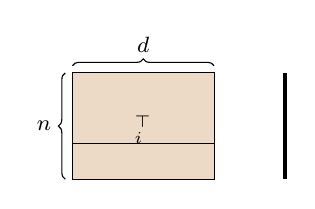
\begin{tikzpicture}[scale=0.9]
        \draw [fill=brown!30] (-2,1.5) rectangle (0,3);
        \draw [color=black] (-2,2) -- (0,2);
        \draw (-1,2.2) node {\mbox{\footnotesize $\x_i^\top$}}; 
        \draw (-2.5,3) node {$\X$}; 
        \draw [decorate,decoration={brace}] (-2,3.1) -- (0,3.1);
        \draw (-1,3.4) node {\mbox{\fontsize{8}{8}\selectfont $d$}}; 
        \draw [decorate,decoration={brace}] (-2.1,1.5) -- (-2.1,3);
        \draw (-2.4,2.25) node {\mbox{\fontsize{8}{8}\selectfont $n$}}; 
        \draw [color=black,line width =0.5mm] (1,1.5) -- (1,3);
        \draw [color=black] (0.75,3) node {$\y$};
      \end{tikzpicture}
    \end{column}
  \end{columns}
  
  
  Moore-Penrose estimator:
  \begin{align*}
    \X^\dagger\y =
      \begin{cases}
        \text{minimum norm solution},& \text{for }n\leq d,\\
        \text{least squares solution},& \text{for }n>d.
      \end{cases}
  \end{align*}
  
  Goal:\quad find\quad$\MSE{\X^\dagger\y}=\E\,\|\X^\dagger\y-\w\|^2$

    Prior work: asymptotics \cite{HMRT19_TR} and upper bounds
    \cite{BLLT19_TR}
    
  \textcolor{red}{No closed form expressions, even for
    $\mu=\Nc(\vec{0},\Sigmab)$!}
\end{frame}

\begin{frame}
  \frametitle{Main result I: exact non-asymptotic MSE}
  Idea: replace standard i.i.d.~design with a surrogate design
  \begin{align*}
    \underbrace{\X\sim\mu^n}_{\text{i.i.d.}}\qquad\Longrightarrow\qquad
    \underbrace{\Xb\sim S_\mu^n}_{\text{surrogate}} 
  \end{align*}
  \vspace{-2mm}
  \begin{theorem}
\label{t:mse}
Let \ $\Xb\sim S_\mu^n$, \ $\yb_i=\xbb_i^\top\w+\xi$ \ and \
$\Sigmab_\mu=\E_\mu[\x\x^\top]$. Then,
  \begin{align*}
 &\MSE{\Xb^\dagger\ybb} =\\
  &  \begin{cases}
    \sigma^2\,\tr\big((\Sigmab_\mu+\lambda_n\I)^{-1}\big)
    \frac{1-\alpha_n}{d-n}\ +\
\frac{\w^{\top}(\Sigmab_\mu+\lambda_n\I)^{-1}\w}
{\tr((\Sigmab_\mu+\lambda_n\I)^{-1})}(d-n),
& (n<d),\\
\sigma^2\, \tr(\Sigmab_\mu^{-1}),& (n=d),\\
\sigma^2\,\tr(\Sigmab_\mu^{-1})\frac{1-\beta_n}{n-d},&(n>d),
\end{cases}
  \end{align*}
  where
  $n=\tr((\Sigmab_\mu+\lambda_n\I)^{-1}\Sigmab_\mu)$, \
  $\alpha_n=\frac{\det(\Sigmab_\mu)}{\det(\Sigmab_\mu+\lambda_n\I)}$,
\ $\beta_n=\ee^{d-n}$.
\end{theorem}
\end{frame}

\begin{frame}
  \frametitle{Isotropic features: double descent curve}
  $\X\sim\mu^n$ \ - standard Gaussian design, $\mu=\Nc(\vec{0},\I)$, $d=100$
  \pause
      \begin{align*}
        \MSE{\X^\dagger\y} =
        \begin{cases}
          \frac{\sigma^2n}{d-n-1} + \|\w\|^2\frac{d-n}{d},&(n<d-1)\\
          \frac{\sigma^2d}{n-d-1},&(n>d+1)
        \end{cases}\quad(\text{let }\|\w\|=1)
      \end{align*}
      \pause\vspace{-2mm}
      \begin{figure}
          \centering
          \includegraphics[width=0.7\textwidth]{Figures/descent/descent-isotropic.pdf}
      \end{figure}
\end{frame}

\begin{subframe}
  \frametitle{Gaussian features: effect of spectral decay}
  $\X\sim\mu^n$ \ - multivariate Gaussian design,
  $\mu=\Nc(\vec{0},\Sigmab)$, $d=100$\\
$\Sigmab$ \ - exponentially decaying eigenvalues, condition
number $\kappa$
\pause
\begin{align*}
\MSE{\X^\dagger\y}\ =\ ?
  \end{align*}
  \pause \vspace{-3mm}
  \begin{figure}
      \centering
      \includegraphics[width=0.7\textwidth]{Figures/descent/descent-full}
  \end{figure}
\end{subframe}

\begin{subframe}
  \frametitle{Gaussian features: effect of model complexity}
    $\X\sim\mu^n$ \ - multivariate Gaussian design,
  $\mu=\Nc(\vec{0},\Sigmab)$, $n=100$\\
$\Sigmab$ \ - exponentially decaying eigenvalues, condition
number $\kappa$
\begin{align*}
\MSE{\X^\dagger\y}\ =\ ?
  \end{align*}\vspace{-3mm}
  \begin{figure}
      \centering
    \includegraphics[width=0.7\textwidth]{Figures/descent/descent-model}
  \end{figure}
\end{subframe}

\begin{frame}
  \frametitle{Main result II: implicit regularization of minimum norm}
Why does this \textit{unregularized} model learn when $n<d$?\\
  \pause
\textit{Because taking minimum norm induces
  $\ell_2$-regularization.}
\vspace{2mm}
\pause
\begin{theorem}
Let \ $\Xb\sim S_\mu^n$, \ $\yb_i=y(\x)$ \ and \
$\Sigmab_\mu=\E_\mu[\x\x^\top]$. Then,\pause
 \begin{align*}
    \E\big[\Xb^\dagger\ybb\big] = 
    \begin{cases}
      (\Sigmab_\mu + \lambda_n\I)^{-1}\v_{\mu,y} &\text{for }n<d,\\
        \Sigmab_\mu^{-1}\v_{\mu,y} &\text{for }n \ge d,
    \end{cases}
 \end{align*}
  where \ $n=\tr((\Sigmab_\mu+\lambda_n\I)^{-1}\Sigmab_\mu)$ \ and \ $\v_{\mu,y}=\E_\mu[y(\x)\,\x ]$.
\end{theorem}
\pause
\begin{align*}
  (\Sigmab_{\mu} +  \lambda_{n}\I)^{-1} \v_{\mu,y}
  \ =\ \argmin_{\wbh} \ \E_{\mu,y}\Big[\big(\x^\top\wbh-y(\x)\big)^2\Big]
    + \lambda_n\|\wbh\|^2
\end{align*}
\end{frame}

\begin{frame}
  \frametitle{Implicit regularization}
  Our observations:\\
  \begin{itemize}
    \item Minimum norm induces an $\ell_2$-regularizer:
      $\lambda_n\|\wbh\|^2$\pause
\item Sample size is effective dimension:
  $n=\tr((\Sigmab_\mu+\lambda_n\I)^{-1}\Sigmab_\mu)$
  \end{itemize}\pause
%\vspace{5mm}

~\hspace{-0.8cm}\includegraphics[width=0.57\textwidth]{Figures/descent/descent-bias}\nobreak\includegraphics[width=0.57\textwidth]{Figures/descent/descent-lambda}
\end{frame}

\begin{frame}
  \frametitle{Consistency of surrogate expressions}
  \begin{align*}
  \MSE{\X^\dagger\y}
  &=\sigma^2\E\big[\tr\big((\X^\top\X)^\dagger\big)\big] +
    \w^{\top}\E\big[\I-\X^\dagger\X\big]\w.
  \end{align*}
  \pause
  \begin{align*}
    \mu=\Nc(\vec{0},\Sigmab)\quad \Longrightarrow\quad
    \begin{cases}
      \X^\top\X&-\quad\text{Wishart distribution}\\
      \X^\dagger\X&-\quad\text{Gaussian projection}
    \end{cases}
  \end{align*}
  \pause
  \begin{conjecture}
  Fix $n/d<1$ and let $\mu=\Nc(\vec{0},\Sigmab )$, where 
  $c\I\preceq\Sigmab\preceq C\I$. Then:\pause
\begin{align*}
\bigg|\frac{\E\big[\tr((\X^\top\X)^\dagger)\big]}{\Vc(\Sigmab,n)} -1\bigg|&=
  O(1/d)\quad\text{for}\quad\Vc(\Sigmab,n)=\frac{1-\alpha_n}{\lambda_n},\\
\onslide<5>{  %\sup_{\w\in\R^d}
  \bigg|\frac{\w^\top\E[\I-\X^\dagger\X]\w}{\w^\top
  \Bc(\Sigmab,n)\w} - 1\bigg| &= O(1/d)\quad\text{for}\quad
  \Bc(\Sigmab,n) = \lambda_n(\Sigmab+\lambda_n\I)^{-1}.}
\end{align*}
\end{conjecture}
\end{frame}

\begin{frame}
  \frametitle{Empirical evidence for the conjecture}
~\hspace{-1cm}\includegraphics[width=1.16\textwidth]{Figures/descent/wishart_var.pdf}\\
~\hspace{-1cm}\includegraphics[width=1.16\textwidth]{Figures/descent/proj_bias.pdf}
\end{frame}

\begin{subframe}
  \frametitle{Surrogate design: rescaling by pseudo-determinant}
  \begin{definition}
    Let $K$ be a random variable over non-negative integers. \\
    A determinantal surrogate design
    $\Xb\sim \Det(\mu,K)$ is defined so that
\begin{align*}
  \E\big[F(\Xb)\big]\  \propto\ \E[\pdet(\X\X^\top)F(\X)]
  \quad\text{for}\quad\X\sim\mu^K.
\end{align*}
\end{definition}
\begin{itemize}
  \pause
\item The proportionality constant is $1/\E[\pdet(\X\X^\top)]$.
\pause
\item To compute it, we let $K$ be a Poisson random variable.
\pause
\item New expectation formulas for $K\sim\Poisson(\gamma)$ and $\X\sim\mu^K$:
\begin{align*}
  \E\big[\det(\X\X^\top)\big]
  &= \ee^{-\gamma}\det(\I+\gamma\Sigmab_\mu)\\
  \E\big[\det(\X^\top\X)\big]
  &= \det(\gamma\Sigmab_\mu)
\end{align*}
\end{itemize}

\end{subframe}

\begin{subframe}
  \frametitle{New technique: \textit{determinant preserving random
      matrices}}
\begin{definition}
A random $d\times d$ matrix $\A$ is \emph{determinant
  preserving} (d.p.) if
\begin{align*}
  \E\big[\!\det(\A_{\Ic,\Jc})\big] =
  \det\!\big(\E[\A_{\Ic,\Jc}]\big)\quad \text{for all }\Ic,\Jc\subseteq
  [d]\text{ s.t. }|\Ic|=|\Jc|.
\end{align*}
\vspace{-7mm}
\end{definition}
\pause
Examples:
  \begin{itemize}
  \item $\A$ has i.i.d.~Gaussian entries  $a_{ij}\sim\Nc(0,1)$\pause    
  \item $\A = s\Z$, where $s$ is random and $\Z$ is a fixed,
    rank-1 matrix\pause
    \item $\A=\X^\top\X$, where $\X\sim\mu^K$ and $K\sim\Poisson(\gamma)$
    \end{itemize}
    \pause
  \begin{theorem}[closure properties]
    If $\A,\B$ are d.p.~and independent, then $\A+\B$ and $\A\B$ are
    also d.p.
  \end{theorem}
\end{subframe}